\chapter{Thrust 4: Visualization Environment}\label{chap:thrust4}

The fidelity and volume of data that can be provided by a discrete facility,
discrete material object agent-based fuel cycle simulator opens the door for a
richer visualization experience.  The fundamental transaction data, as
described in Chapter \ref{chap:thrust3}, can be considered most abstractly as
the mass of each transaction sparsely mapped onto a five-dimensional domain:
time, sending facility, receiving facility, material ID, nuclide.  The
simplest visualizations are formed from filtering this data set on some
domains and aggregating it on other domains.  For example, the total
time-dependent flow between two facilities is found by filtering the
sending/receiving facility domains with those two facilities, and aggregating
over the material id and nuclide domains.  Being able to easily select the
filters and aggregations can enable data exploration that may not be natural
through more typical spreadsheet based data analysis environments.  Additional
power can be derived from examining different linked visualizations in which
the filter and aggregation operations on one are reflected on the other.

Thrust 4 was led by Yarden Livnat at the University of Utah, to develop a
complete visualization environment that can enable a richer data exploration
experience.  The lack of a robust \gls{ngfcs} in the early stages of the
project limited the scope of this thrust.  While this thrust originally aimed
to explore different visualization modes for different levels of nuclear fuel
cycle expertise, it focused instead on providing visualization capability for
\Cyclus for developers and expert users.  This was driven, in part, by a need
for \Cyclus developers to visualize results during the development process.
This thrust was also somewhat hampered by a lack of real-world analysis needs
within the project.  Without interesting output analysis, it was difficult to
motivate advanced visualization needs despite the availability of a richer
data set.

In order to simplify distribution across many types of computing systems, and
to take advantage of existing high quality visualization toolsets and user
interface widgets, the JavaFX software platform was selected for this thrust.
This decision ultimately drove the software platform decision of Thrust 2, as
well.  JavaFX is a freely available platform that is supported on a wide
variety of computing systems.

\section{Cyclist}

The tool for data visualization is named Cyclist, and ultimately incorporated
the Cycic model building environment as a single platform-independent tool.
It is a stand-alone application that can read \Cyclus databases from the local
computer or access a remote execution server to download and access a
database.  Upon loading a database, Cyclist checks for the existence of an
inventory table in the database, as described in section \ref{sec:fund_data}
and reconstructs the inventory if not present using Cyan-based methods.
Cyclist then offers a list of database tables to the user from which to select
data to visualize.  Once a table is selected, each of the columns of that
table are offered in a separate list as specific data to include in a
visualization.  The other columns in that table become available for other
operations such as aggregation or filtering.

\subsection{Workspaces}

The visualization environment is arrange in workspaces, each of which may
contain multiple individual visualizations.  Some characteristics of the
workspace apply to all the visualizations in that workspace, allowing for
operations to be applied to a workspace such that its effects are reflected in
all visualizations simultaneously.  Multiple workspaces can be opened
simultaneously, each with different settings and operations applied.  A
workspace can be duplicated, thus allowing for largely the same
visualizations, but with slightly different operations or slightly different
parameters for those operations.

\subsection{Drag \& Drop}

Most operations in a workspace are implemented by a drag-and-drop interaction
mode.  Once a new chart has been created, the a database table columns can be
dragged and dropped to populate the X and Y axes, as well as the ``Group by''
entry which enables aggregation and filtering (see the next section).
Depending on the data types of the columns chosen for the X and Y axes, a set
of operations will be offered that can be applied to that data.  For example,
in some circumstances it may be logical to sum the value in the Y axis for
each point on the X axis. The type of plot is automatically adapted to the
type of data being plotted.  For a continuous variable, e.g. Time, the plot
will be a typical x-y scatter/line plot.  For a discrete variable,
e.g. Prototype, the plot will be a column/bar chart.

\subsection{Aggregation \& Filters}

Additional columns can be dragged into the ``Group by'' entry to create
categories for the operation being applied to the Y axis data.  For example,
if the Y-axis data is being summed over all rows for each X axis point, the
addition of a grouping field will separate the single sum into multiple sums,
each associated with a different result in the grouping column.

In a similar fashion, additional fields can be dragged into the title bar of
the plot to create an opportunity for filtering.  For each field in the
filtering bar, a new user interface appears that allows the user to select
from the values in that field.  For fields that represent discrete quantities,
the filter interface appears as a set of checkboxes and the user can select
which values are shown or not.  For fields that are represented as continuous
quantities, the users specifies the maximum and minimum, either with a slider
or with text boxes depending on the required precision.  It is possible, but
not required, for fields to be used for both aggregation and filtering,
increasing the flexibility of generating plots.

Figure \ref{fig:plot-01-07} shows a sample plot with aggregation across
multiple fields and filtering across multiple fields.  In this case, the total
quantity of material in inventory as a function of time.  Since there may be
many discrete inventories, the Y-axis value is summed over all possible
inventories.  Without grouping, this would result a single curve on the plot.
However, in this problem, the quantities are grouped by both Prototype (of
which there are three) and Nuclide (of which there are four).  Therefore,
there is a single curve for each combination of Prototype and Nuclide.  This
plot also includes filtering by Prototype, Nuclide and Time.  The user has
selected to see all Prototypes, but only the fissile nuclides.  Finally, the
user has asked to see only the first 60 time steps.  Since Time also defines
the X-axis, this serves to zoom in the plot to those 60 time steps.

\begin{figure}[htbp]
  \centering
  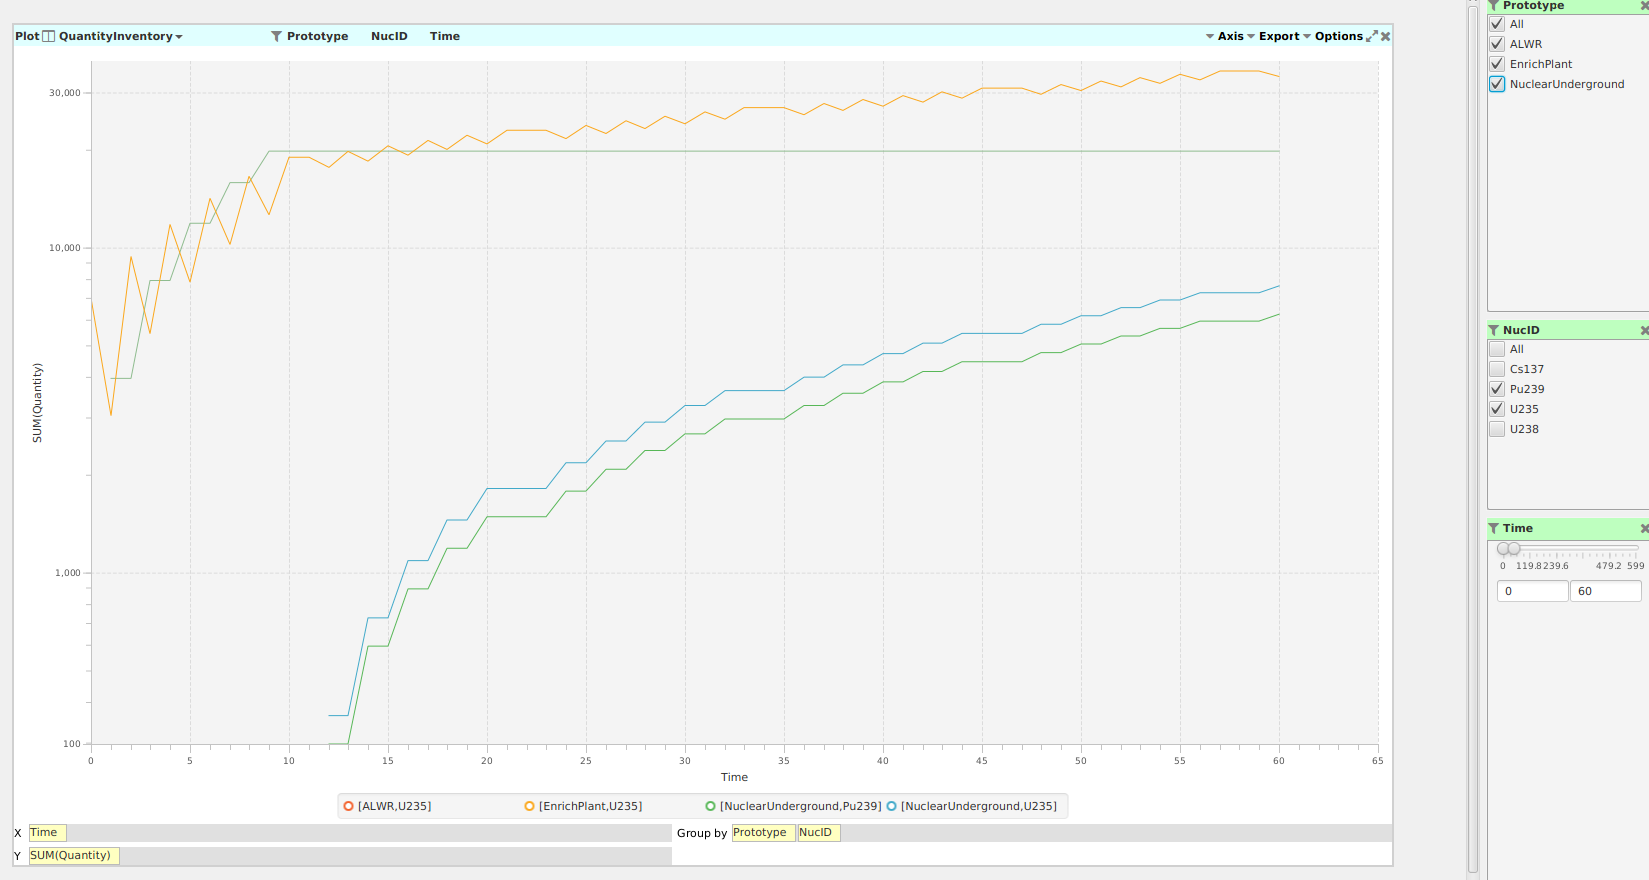
\includegraphics[width=\columnwidth]{./images/plot-01-07}
  \caption{A typical plot showing the quantity of material inventory at each
    point in time.  This case shows the application of a SUM operation to the
    Y-axis data, grouping of the results by Prototype and Nuclide, and
    subsequent filtering by Prototype, Nuclide and Time.  Since Time is a
    continuous variable, the user interface for this filter is different.  Since
    Time is the X-axis variable, its filter is applied differently.  }
  \label{fig:plot-01-07}
\end{figure}

\subsection{Extensibility}

Since it is possible for many tables to exist in the \Cyclus output database,
Cyclist shows only a default set of tables in its interface.  There is also a
mechanism, however, to add any table, including custom tables, to that list.
Thus, if an archetype developer adds a custom table to the database it is
still possible to use Cyclist to visualize the data it contains with no
changes to Cyclist.

\section{Custom Visualization: Material Flows}

Although the primary visualization modes in Cyclist are based on
well-understood x-y plots, there was also a desire to implement application
specific visualizations to support fuel cycle analysis.  Following the network
flow model that underlies the \Cyclus, a material flow visualization was
created to demonstrate an interactive and exploratory visualization mode.

As shown in Figure \ref{fig:flow-01-05}, this visualization provides a way to
examine both total flows and time dependent flows between sets of agents.
Both the sender and receiver can be used to specify archetypes, prototypes, or
individual agents, whether regions, institutions or facilities.  Multiple
pairs of flows can be included for comparison purposes.  As each pair is added
to the flow map, its cumulative flow is added to the strip chart below.  The
checkboxes on the let allow for filtering by the commodity and by the nuclide.
Finally, a time window can be specified over which to sum the flow as reported
on the flow diagram.

\begin{figure}[htbp]
  \centering
  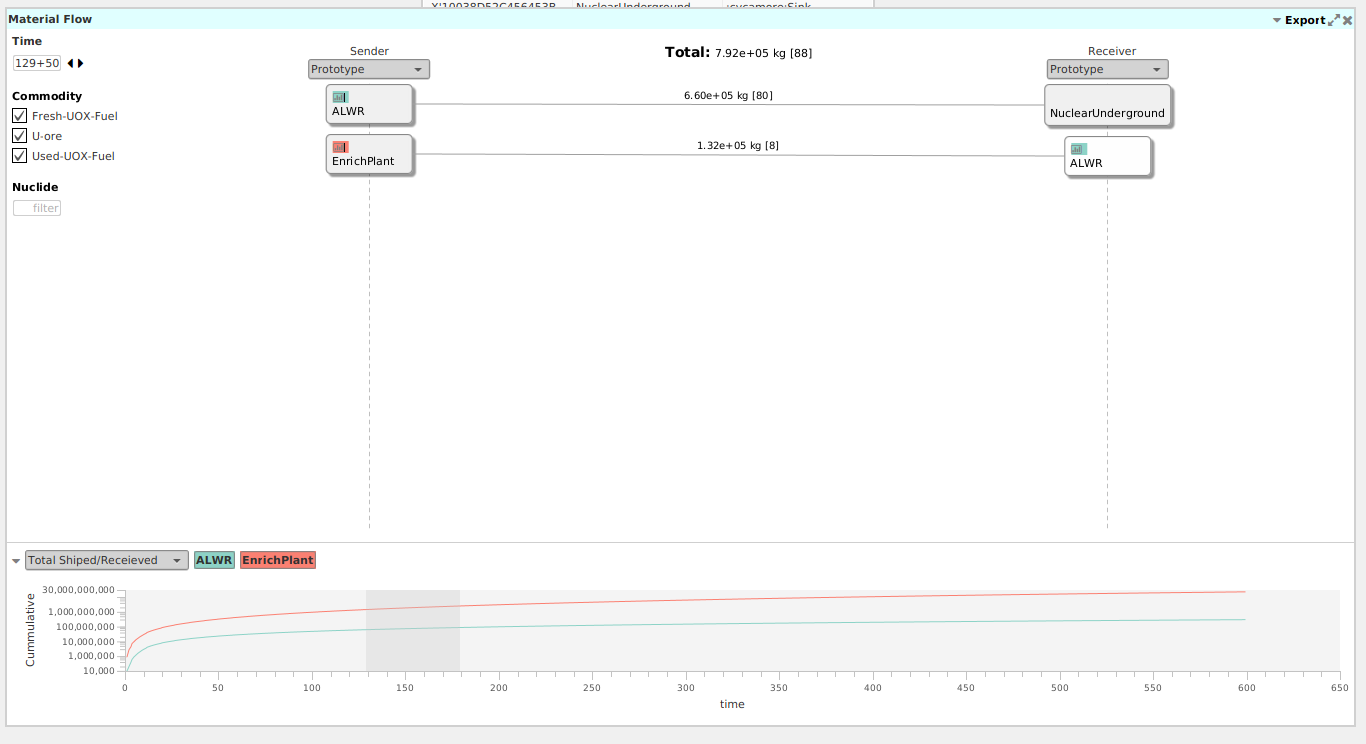
\includegraphics[width=\columnwidth]{./images/flow-01-05}
  \caption{A flow visualization shows the total flow between different pairs of
    prototypes, aggregating over all agents that share that prototype.  The
    upper pane shows the sender receiver pairs while the lower pane shows the
    cumulative flow as a function of time.  The quantity shown in the upper
    pane is the total flow contained in the window indicated in gray from time
    step 129-179. }
  \label{fig:flow-01-05}
\end{figure}

Different visual representations of this flow information have been
conceptualized for future development, including a map-based view in the event
of trade among many regions, or a graph-based view for representing flows
throughout the whole fuel cycle.

\section{Limitations}

There were some limitations identified during the development of Cyclist.
First and foremost, as \Cyclus simulations became more complicated, the volume
of data began to become an obstacle.  This was true both in terms of accessing
the database file as well as managing the data in memory.  This is
particularly true for the operation that builds an inventory table from the
transaction tables.  Furthermore, there is growing interest in processing
results for 100's or 1000's of separate but related \Cyclus runs either due to
parametric sweeps, sensitivity studies, or optimization capability.  The
current Cyclist infrastructure is not well suited for such applications.

In addition, since the beginning of this project, large investments have been
made by various third parties in the technology for Javascript-based software.
Visualization solutions and user interface widgets in Javascript have achieved
a quality that surpasses the JavaFX version, propelled by rapid development of
web apps for a variety of computing platforms, particularly mobile.  A new
project has begun that is expected to replace Cyclist with a Javascript based
interface and rely more heavily on intermediate computing capability to
process results before reaching the device that will actually display the
results.

\section{Summary}

A dedicated, open source visualization tool was developed to facilitate the
display of \Cyclus databases in creative ways.  This tool was designed with an
advanced user in mind - one who could interpret the names of fields and tables
in the output data base.  The basic framework for this visualization tool
could be used for more creative visual representations and to craft simplified
tools for different categories of users.  The Cycic model building tool was
integrated into Cyclist so that users had a uniform experience in both
generating their model and analyzing the results.  Both tools support remote
execution (see Chapter \ref{chap:thrust5}) and therefore Cyclist became a
convenient way to distribute access to \Cyclus without requiring users to
install it independently.

